% !TeX root = ../main.tex
%
\chapter{Swing-Up Design}
This chapter contains a swing-up design for the twin pendulum system. As for the cart pendulum system in \textit{Part 1} the design is based on \cite{kjAastrom}. The presented approach is similar to the sat-based energy controller, the final design from \textit{Part 1}. Detailed nonlinear analysis is left out here since this design exploits the same principals as for the final cart pendulum swing-up controller in \textit{Part 1}.\\
Both pendulums are started in $\pi$ at rest and the design is based on the pendulum energies in the coordinate system fixed to the cart, thus reducing the generalized coordinates to,
%
\begingroup\makeatletter\def\f@size{10}\check@mathfonts
\def\maketag@@@#1{\hbox{\m@th\normalsize\normalfont#1}}%
\begin{flalign}
  &
  \begin{cases}
    x_{p_1} =  - l_1 \sin \theta_1 \\
    y_{p_1} =  l_1 + l_1 \cos \theta_1
  \end{cases}
  %\hspace{10pt}
  \begin{cases}
    x_{p_2} =  - l_2 \sin \theta_2 \\
    y_{p_2} =  l_1 + l_2 \cos \theta_2
  \end{cases}
  %\label{eq:excessiveToGeneralized2} \\
  \begin{cases}
    \dot{x}_{p_1} =  - l_1 \cos \theta_1 \dot{\theta}_1 \\
    \dot{y}_{p_1} =  -l_1 \sin \theta_1 \dot{\theta}_1
  \end{cases}% &
  %\hspace{10pt}
  \begin{cases}
    \dot{x}_{p_2} = - l_2 \cos \theta_2 \dot{\theta}_2 \\
    \dot{y}_{p_2} = -l_2 \sin \theta_2 \dot{\theta}_2 \ \ \ \ .
  \end{cases}\hspace{-1cm}
  \label{eq:excessiveToGeneralizedDerivatives2}
  &\\ \nonumber
\end{flalign}\endgroup \vspace{-44pt}

Since the energies of the two pendulums are described in a local coordinate system fixed to the cart, there is no cross-coupling, thus the energies are independent of one another,
%
\begin{align}
  E_{p_1} &= m_1 g y_{p_1} + \tfrac{1}{2} m_1 \dot{x}_{p_1}^2 + \tfrac{1}{2} m_1 \dot{y}_{p_1}^2             \label{eq:pendulum1Energy} \\
  E_{p_2} &= m_2 g y_{p_2} + \tfrac{1}{2} m_2 \dot{x}_{p_2}^2 + \tfrac{1}{2} m_2 \dot{y}_{p_2}^2   \ \ \ ,   \label{eq:pendulum2Energy}
\end{align}
%
and in generalized coordinates,
\begin{align}
  E_{p_1} &= \tfrac{1}{2} J_1 \dot{\theta}_1^2 + m_1 g l_1 (\cos \theta_1 + 1)             \label{eq:pendulum1EnergyGeneralized} \\
  E_{p_2} &= \tfrac{1}{2} J_2 \dot{\theta}_2^2 + m_2 g (l_2 \cos \theta_2 + l_1) \ \ \ ,   \label{eq:pendulum2EnergyGeneralized}
\end{align}
%
where the inertia $J_1 = m_1 l_1^2$ and $J_2 = m_2 l_2^2$ and the energy in equilibrium for each pendulum is,
\begin{align}
  & E_{eq_1} = 2 m_1 g l_1 \ \ \ , \ \ \ \ E_{eq_2} = m_2 g (l1 + l2)   \ \ \ ,    \label{eq:eqEnergyTwin}
\end{align}
%
such that,
\begin{align}
  E_{\Delta_1} &= E_{p_1} - E_{eq_1} = \tfrac{1}{2} J_1 \dot{\theta}_1^2 + m_1 g l_1 (\cos \theta_1 - 1)             \label{eq:pendulum1EnergyError} \\
  E_{\Delta_2} &= E_{p_2} - E_{eq_2} =  \tfrac{1}{2} J_2 \dot{\theta}_2^2 + m_2 g l_2 (\cos \theta_2 - 1) \ \ \ .   \label{eq:pendulum2EnergyError}
\end{align}
%
Choosing the function candidate,
\begin{align}
  V(\theta_1, \theta_2, \dot{\theta}_1, \dot{\theta}_2) &= \tfrac{1}{2} E_{\Delta_1} ^2 + \tfrac{1}{2} E_{\Delta_1} ^2 \ \ \ ,   \label{eq:lyapunovCandidateTwin} 
\end{align}
%
and with the dynamics given by,
\begin{align}
  J \ddot{\theta} &= m_1 l_1 \cos \theta_1 a_c + m_1 g l_1 \sin \theta_1          \label{eq:pendulum1DynamicsTwin} \\
  J \ddot{\theta} &= m_2 l_2 \cos \theta_2 a_c + m_2 g l_2 \sin \theta_2 \ \ \ ,  \label{eq:pendulum2DynamicsTwin}
\end{align}
%
the derivative of $V$ is evaluated along trajectories of the system,
\begin{align}
  \dot{V} &= E_{\Delta_1} \dot{E}_{\Delta_1} + E_{\Delta_2} \dot{E}_{\Delta_2}
  \label{eq:lyapunovDerivativeTwin1} \\ 
  \dot{V} &=
  E_{\Delta_1} ( J_1 \dot{\theta}_1 \ddot{\theta}_1 - m_1 g l_1 \sin \theta_1 \dot{\theta}_1 )  \nonumber \\
  &+
  E_{\Delta_2} ( J_2 \dot{\theta}_2 \ddot{\theta}_2 - m_2 g l_2 \sin \theta_2 \dot{\theta}_2 ) 
  \label{eq:lyapunovDerivativeTwin2} \\
  \dot{V} &= E_{\Delta_1} ( \dot{\theta}_1 ( m_1 l_1 \cos \theta_1 a_c + m_1 g l_1 \sin \theta_1 )  - m_1 g l_1 \sin \theta_1 \dot{\theta}_1 ) \nonumber \\
  &+
  E_{\Delta_2} ( \dot{\theta}_2 ( m_2 l_2 \cos \theta_2 a_c + m_2 g l_2 \sin \theta_2 )  - m_2 g l_2 \sin \theta_2 \dot{\theta}_2 )
  \label{eq:lyapunovDerivativeTwin3} \\
  \dot{V} &= G a_c   \ \ \ ,  \label{eq:lyapunovDerivativeTwin4}
\end{align}
%
where,
\begin{align}
  G &= m_1 l_1 E_{\Delta_1} \cos \theta_1 \dot{\theta}_1 +  m_2 l_2 E_{\Delta_2} \cos \theta_2 \dot{\theta}_2  \ \ \ .  \label{eq:lyapunovDerivativeTwinG}
\end{align}
Following control law for the pivot point acceleration, $a_c$, is chosen such that $\dot{V}$ is negative semi-definite,
\begin{align}
  a_c &= sat( -k G ) \ \ \ ,  \label{eq:twinSwingControl1}
\end{align}
where $k$ is a tuning parameter and,
\begin{align}
  \text{sat}(s) &=
  \begin{cases}
    \ \ s                           & \ \  | s |  \leq a_{max} \\
    \ \ \mathrm{sgn}( s )\ a_{max}  & \ \  | s |  >  a_{max} \ \ \ .
  \end{cases}
  \label{eq:satuationFunctionTwin}
\end{align}
%
This control law exhibits the same properties as the first design in \textit{Part 1}, thus the largest invariant set also contains the stable equilibrium at $\pi$, which is the starting position of the pendulums. For this design, the issue is solved by applying a large current, $i_{max}=$ \SI{4.58}{A}, for \SI{0.1}{s} before initiating the swing-up sequence, thus starting at some initial values for which the control signal is different from zero.\\
The controller for cart position from \textit{Part 1} is used unchanged in this design.
%
\begin{figure}[H]
  \hspace{-10pt}
  \captionbox 
  {
    The mechanical energy for each pendulum approach that of their respective equilibrium points shown here by difference in energy.
    \label{fig:Edelta_twinSwing}
  }
  {
    \hspace{-1cm}
    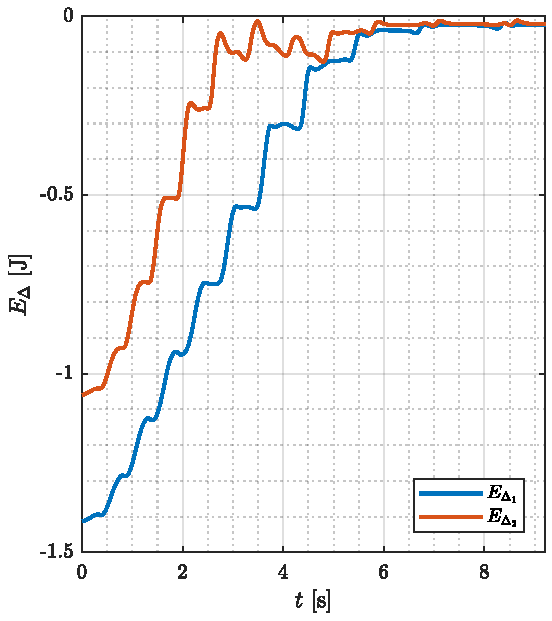
\includegraphics[width=.448\textwidth]{figures/Edelta_twinSwing}
  }
  \hspace{20pt}
  \captionbox 
  {
    Both pendulums of the twin system successfully reaches their heteroclinic orbit. Notice how the shorter pendulum (red) reaches higher angular velocity at its orbit than the longer pendulum (blue), which makes sense as the shorter pendulum has a higher frequency.
    \label{fig:phase_twinSwing}
  }
  {
    \hspace{-1cm}
    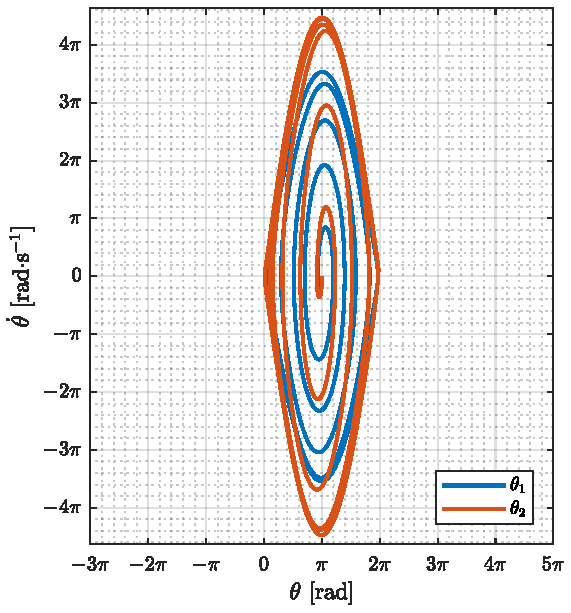
\includegraphics[width=.46\textwidth]{figures/phase_twinSwing}
  }
\end{figure}
%
The design is implemented for simulation, see \autoref{fig:Edelta_twinSwing} and \ref{fig:phase_twinSwing}, effectively driving the energy differences to zero and reaching a heteroclinic orbit for both pendulums. In these simulations the gain is chosen to $k=16$ and \SI{.022}{J} is added to the energy references to reach orbit.
%
%
In \autoref{fig:theta_twinSwing} and \ref{fig:ani_twinSwing} it is seen that though the two pendulums reach their heteroclinic orbits, they do not necessarily reach equilibrium simultaneously. However, using a wrapped version of the angles, same as in \textit{Part 1}, it is possible to catch both pendulums while in opposing equilibrium points. Such a scenario is seen most clearly at the end in \autoref{fig:theta_twinSwing} and \ref{fig:ani_twinSwing} about 11 swings into the simulation.
\begin{figure}[H]
  \hspace{-10pt}
  \captionbox 
  {
    Due to different lengths of the two pendulums the frequencies are different thus the signals drift compared to one another.
    \label{fig:theta_twinSwing}
  }
  {
    \hspace{-1cm}
    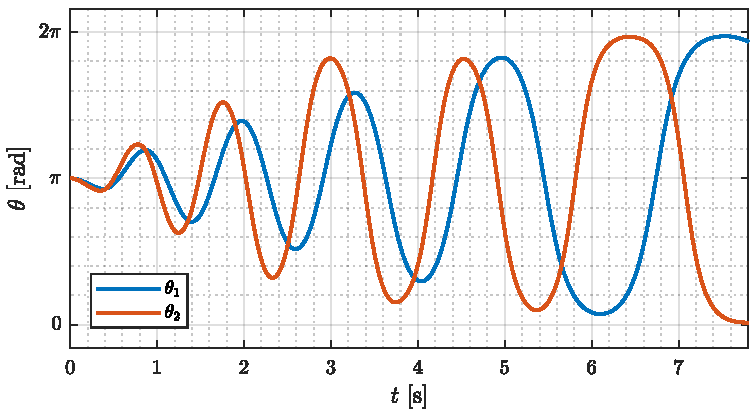
\includegraphics[width=.46\textwidth]{figures/theta_twinSwing}
  }
  \hspace{20pt}
  \captionbox 
  {
    The two pendulums meet in upright position but at opposing equilibrium points.
    \label{fig:ani_twinSwing}
  }
  {
    \hspace{-1cm}
    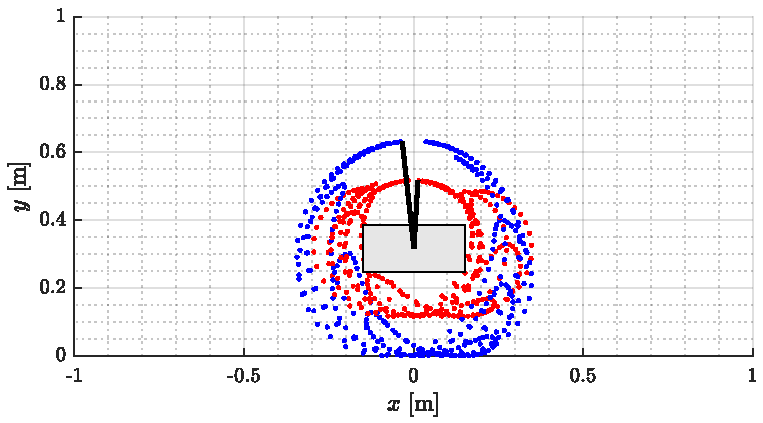
\includegraphics[width=.46\textwidth]{figures/ani_twinSwing}
  }
\end{figure}
%
The control signal used to obtain the behavior in these simulations are shown in \autoref{fig:ia_twinSwing}.
%
\begin{figure}[H]
  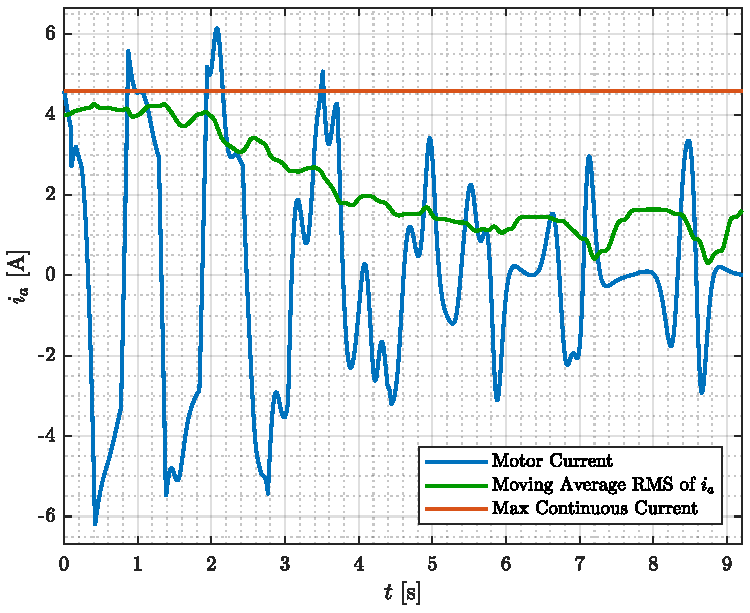
\includegraphics[width=.5\textwidth]{figures/ia_twinSwing}
  \caption{The control signal required for the twin pendulum swing-up behavior simulated in this chapter is within the limits of the motor.}
  \label{fig:ia_twinSwing}
\end{figure}
%
\autoref{fig:x_twinSwing} and \ref{fig:xDot_twinSwing} shows that the position control from \textit{Part 1} also works well with the twin pendulum swing-up design.
\begin{figure}[H]
  \hspace{-10pt}
  \captionbox
  {
    The position control design used in \textit{Part 1} also shows good results for the twin pendulum.
    \label{fig:x_twinSwing}
  }
  {
    \hspace{-1cm}
    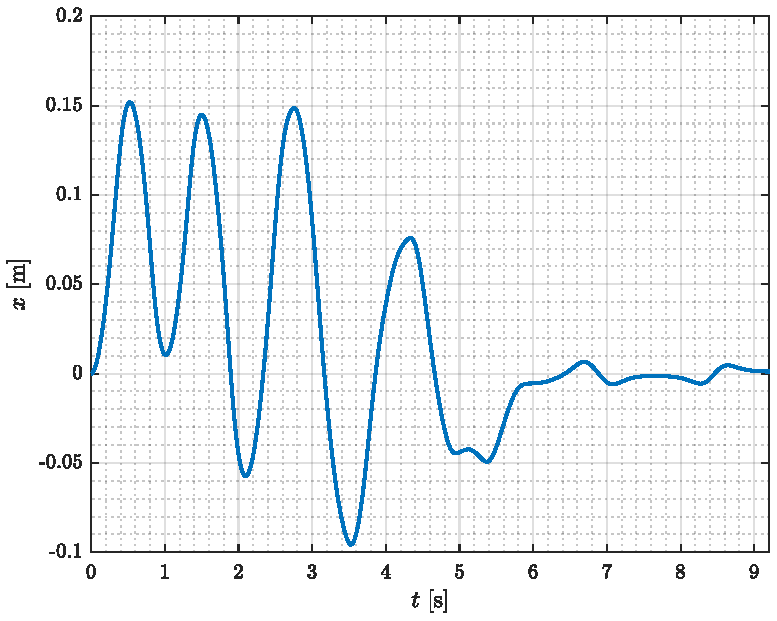
\includegraphics[width=.4\textwidth]{figures/x_twinSwing}
  }
  \hspace{20pt}
  \captionbox 
  {
    Both states, $x$ and $\dot{x}$, are successfully brought to around zero while still allowing the swing-up controller to maintain orbit.
    \label{fig:xDot_twinSwing}
  }
  {
    \hspace{-1cm}
    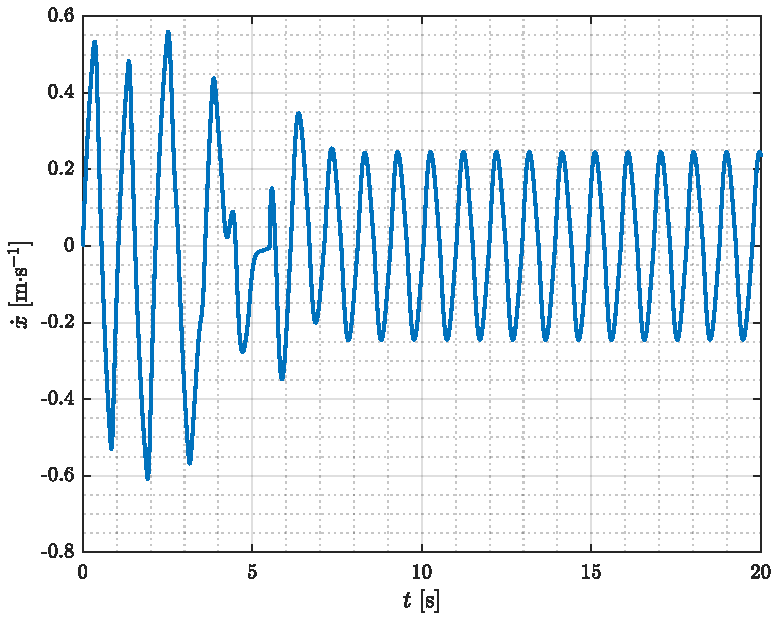
\includegraphics[width=.4\textwidth]{figures/xDot_twinSwing}
  }  
\end{figure}
%
%
%\begin{figure}[H]
%  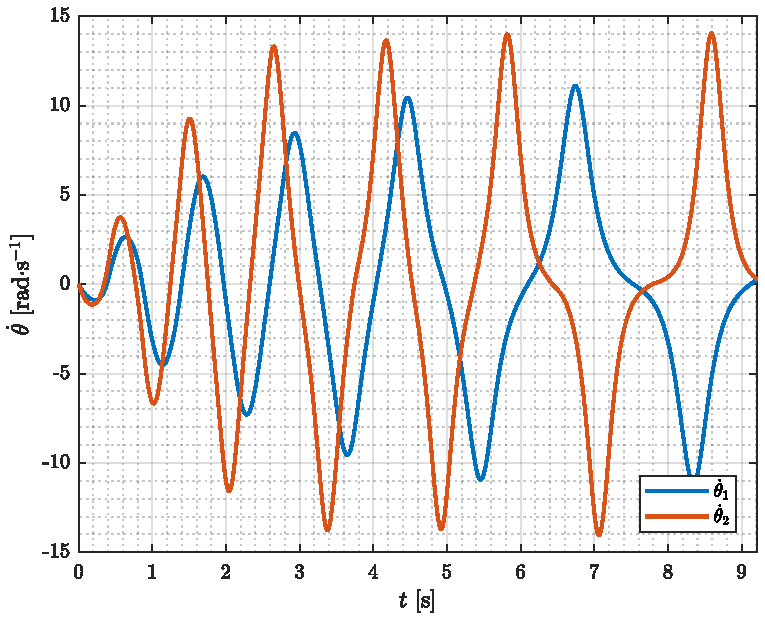
\includegraphics[width=.6\textwidth]{figures/thetaDot_twinSwing}
%  \caption{thetaDotTwinSwing}
%  \label{fig:thetaDot_twinSwing}
%\end{figure}
%\begin{figure}[H]
%  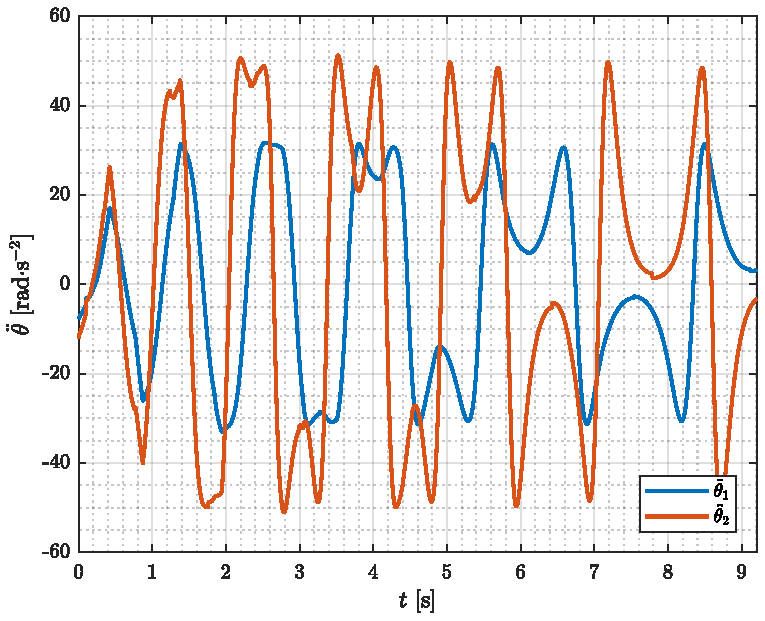
\includegraphics[width=.6\textwidth]{figures/thetaDotDot_twinSwing}
%  \caption{thetaDotDotTwinSwing}
%  \label{fig:thetaDotDot_twinSwing}
%\end{figure}
%\begin{figure}[H]
%  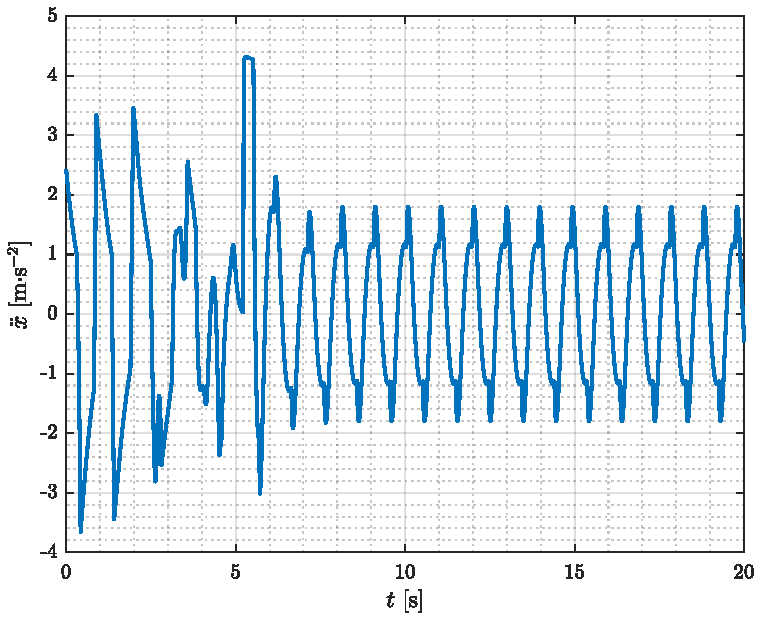
\includegraphics[width=.6\textwidth]{figures/xDotDot_twinSwing}
%  \caption{xDotDotTwinSwing}
%  \label{fig:xDotDot_twinSwing}
%\end{figure}